% To do:
% Perplexity details, Word Error Rate for training (method section).
% The norm of different layers after training and before training
% Our framework is flexible. (abstract?)
% Do we need to say more about the R@5, R@10 for flickr-30K? (experiment)
% Details of the training: (model description? exp? prefer experiments)
%  1. Number of words in the dictionary
%  2. Word error rate
%  3. Training time
% Finetuning the networks? (future works)

\section{Experiments}

\subsection{Datasets}
We test our method on three benchmark datasets with sentence level annotations: IAPR TC-12 \cite{grubinger2006iapr}, flickr 8K \cite{rashtchian2010collecting}, and flickr 30K \cite{hodoshimage}.

Here are some statistics and our experimental settings for the three datasets:

\textbf{IAPR TC-12 Benchmark}  This dataset consists of around 20,000 images taken from locations around the world.
This includes images of different sports and actions, people, animals, cities, landscapes, and so on.
For each image, they provide at least one sentences annotations.
On average, there are about 1.7 sentences annotations for one image.
We adopt the publicly available separation of training and testing set as previous works \cite{GVS10a,kiros2013multimodal}.
There are 17,665 images for training and 1962 images for testing.

\textbf{Flickr8K Benchmark}  This dataset consists of 8,000 images extracted from Flickr.
For each image, they provide five sentences annotations.
The grammar for the annotations of this dataset is simpler than those of the IAPR TC-12 dataset.
We adopt the standard separation of training, validation and testing set which is provided by the dataset.
There are 6,000 images for training, 1,000 images for validation and 1,000 images for testing.

\textbf{Flickr30K Benchmark}  This dataset is a recent extension of Flickr8K.
It consists of 158,915 crowd-sourced captions describing 31,783 images.
So for each image, they also provide five sentences annotations.
The grammar and style for the annotations of this dataset is similar to Flickr8K.
We follow the previous work \cite{karpathy2014fragment} which used 1,000 images for testing.
This dataset, as well as the Flick8K dataset, is mainly used for the image-sentence retrieval tasks and there is not public available results of methods for generating novel sentence descriptions.

\subsection{Experiments settings}

Our model can be used for three tasks: 1) Sentences generation; 2) Sentence retrieval (retrieval top relevant sentences to the given image); 3) Image retrieval (retrieval top relevant images to the given sentence);

\subsubsection{Evaluation metrics for sentence generation}
Following previous works, we use sentence perplexity and BLEU score \cite{papineni2002bleu,lin2004automatic} as the evaluation metrics.
BLEU score was originally designed for automatically machine translation where the task is to give a score to a translated sentences given several references sentences.
We can treat the sentence generation task as the "translation" of the content of image to sentences.
The drawback of using BLEU in our task is that for some images, the reference sentences might not contains all the elements and content in the image and the BLEU score might penalize the arguably correct generated sentences, though it remains as the standard evaluation metric for sentence generation methods for image.
To conduct a fair comparison, we adopt the same sentence generation steps and experiment settings as \cite{kiros2013multimodal}, and generate as many words as there are in the reference sentences.
Note that our model actually do not need to know the length of the reference sentence because we add a end sign "\#\#END\#\#" at the end of every training sentences and we can stop the generation process when our model outputs the word "\#\#END\#\#".

\subsubsection{Evaluation metrics for sentence retrieval and image retrieval}
\label{sec:EvaRet}
For Flickr8K and Flickr30K datasets, we adopted the same evaluation metrics as previous works \cite{socher2014grounded,frome2013devise,karpathy2014fragment} for both the tasks of sentences retrieval and image retrieval.
They used R@K (K = 1, 5, 10), which is the recall rate of the first groundtruth sentences (sentence retrieval task) or images (image retrieval task) as the measurements.
Higher R@K usually means better retrieval performance of different methods.
Since we care most of the top retrieved results, the R@K with smaller K is more important than those with larger K.
In addition to R@K, they used the Med r, which is the median rank of the first groundtruth sentences (sentence retrieval task) or images (image retrieval task).
Lower Med r usually means better performance.

For IAPR TC-12 datasets, we adopt exactly the same evualation metrics as \cite{kiros2013multimodal}, which plotted the mean number of matches of the retrieved groundtruth sentences or images with respect to the percentage of the retrieved sentences or images for the testing set.
For sentences retrieval task, \cite{kiros2013multimodal} used a shortlist of 100 images which are the nearest neighbors of specific testing image in the image feature space.
This shortlist makes the task harder because similar images might have similar descriptions and it is often harder to find the subtle difference among the sentences and pick the most suitable one.
Although there is no published R@K score and Med r score for this dataset as the best of our knowledge, we also report these metrics of our method for future comparison.

\subsection{Results on IAPR TC-12}

\begin{table}[htb]
	\centering
\begin{tabular}{l|cccc}
\hline
      & PERP  & B-1   & B-2   & B-3 \\
\hline
BACK-OFF GT2 & 54.5  & 0.323 & 0.145 & 0.059 \\
BACK-OFF GT3 & 55.6  & 0.312 & 0.131 & 0.059 \\
LBL \cite{mnih2007three}  & 20.1  & 0.327 & 0.144 & 0.068 \\
MLBL-B-DeCAF \cite{kiros2013multimodal} & 24.7  & 0.373 & \textbf{0.187} & 0.098 \\
MLBL-F-DeCAF \cite{kiros2013multimodal} & 21.8  & 0.361 & 0.176 & 0.092 \\
Gupta et al. \cite{gupta2012choosing} & /     & 0.15  & 0.06  & 0.01 \\
Gupta \& Mannem \cite{gupta2012image} & /     & 0.33  & 0.18  & 0.07 \\
\hdashline
Ours-RNN-Base & 7.77  & 0.3134 & 0.1168 & 0.0803 \\
Ours-m-RNN & \textbf{6.92} & \textbf{0.3951} & 0.1828 & \textbf{0.1311} \\
\hline
\end{tabular}%
	\caption{Results of generated sentences in the iaprtc-12 dataset. }
	\label{tab:iaprtc_gen}
\end{table}

The results of generated sentences is shown in Table \ref{tab:iaprtc_gen}.
BACK-OFF GT2 and GT3 are n-grams methods with Katz backoff and Good-Turing discounting \cite{chen2000survey,kiros2013multimodal}.
Ours-RNN-Base has the same architecture with our m-RNN model except that we will not input the image features to the network.
It serves as a baseline for our m-RNN model.

To conduct a fair comparison, we followed the same experimental settings of \cite{kiros2013multimodal}, includes the context length to calculate the BLEU score and perplexity.
Please note that the perplexity is calculated according to the conditional probability of the words given all of its previous reference words in the sentences.
Therefore, a strong language model that successfully captures the grammar of sentences can have a low perplexity without the image content. 
Perplexity does not directly correlate to the BLEU score where we need to sample the words from the probability distribution generated by the model.
For example, although for this dataset, our baseline method of RNN can generate a very low perplexity, it failed to generated sentences with high quality since its BLEU score is not very high.
From this perspective, the BLEU score is a better measurement for the generating sentences.

From the experiments, we can see that our m-RNN model performs much better than our baseline RNN model in terms of both perplexity and BLEU score.
It also outperforms the state-of-the-art methods in terms of perplexity, B-1, B-3, and a comparable result for B-2.

For retrieval tasks, as mentioned in Section \ref{sec:EvaRet}, we draw a recall accuracy curve with respect to the percentage of retrieved images (Text to Image) or retrieved sentences (Image to Text) shown in Figure \ref{fig:iaprtc_ret_curve}.
For sentence retrieval task, we used a shortlist of 100 images as the three comparing methods \cite{kiros2013multimodal}.
The first method, bow−decaf, is a strong image based bag-of-words baseline.
The second and the third models are all multimodal deep models.
Our m-RNN model outperforms these three methods by a large margin.

Since there are no publicly available results of R@K and median rank in this dataset, we report R@K scores of our method in table \ref{tab:iaprtc_ret} for future comparisons.

\begin{figure}[htb]
        \centering
        \begin{subfigure}[b]{0.42\textwidth}
                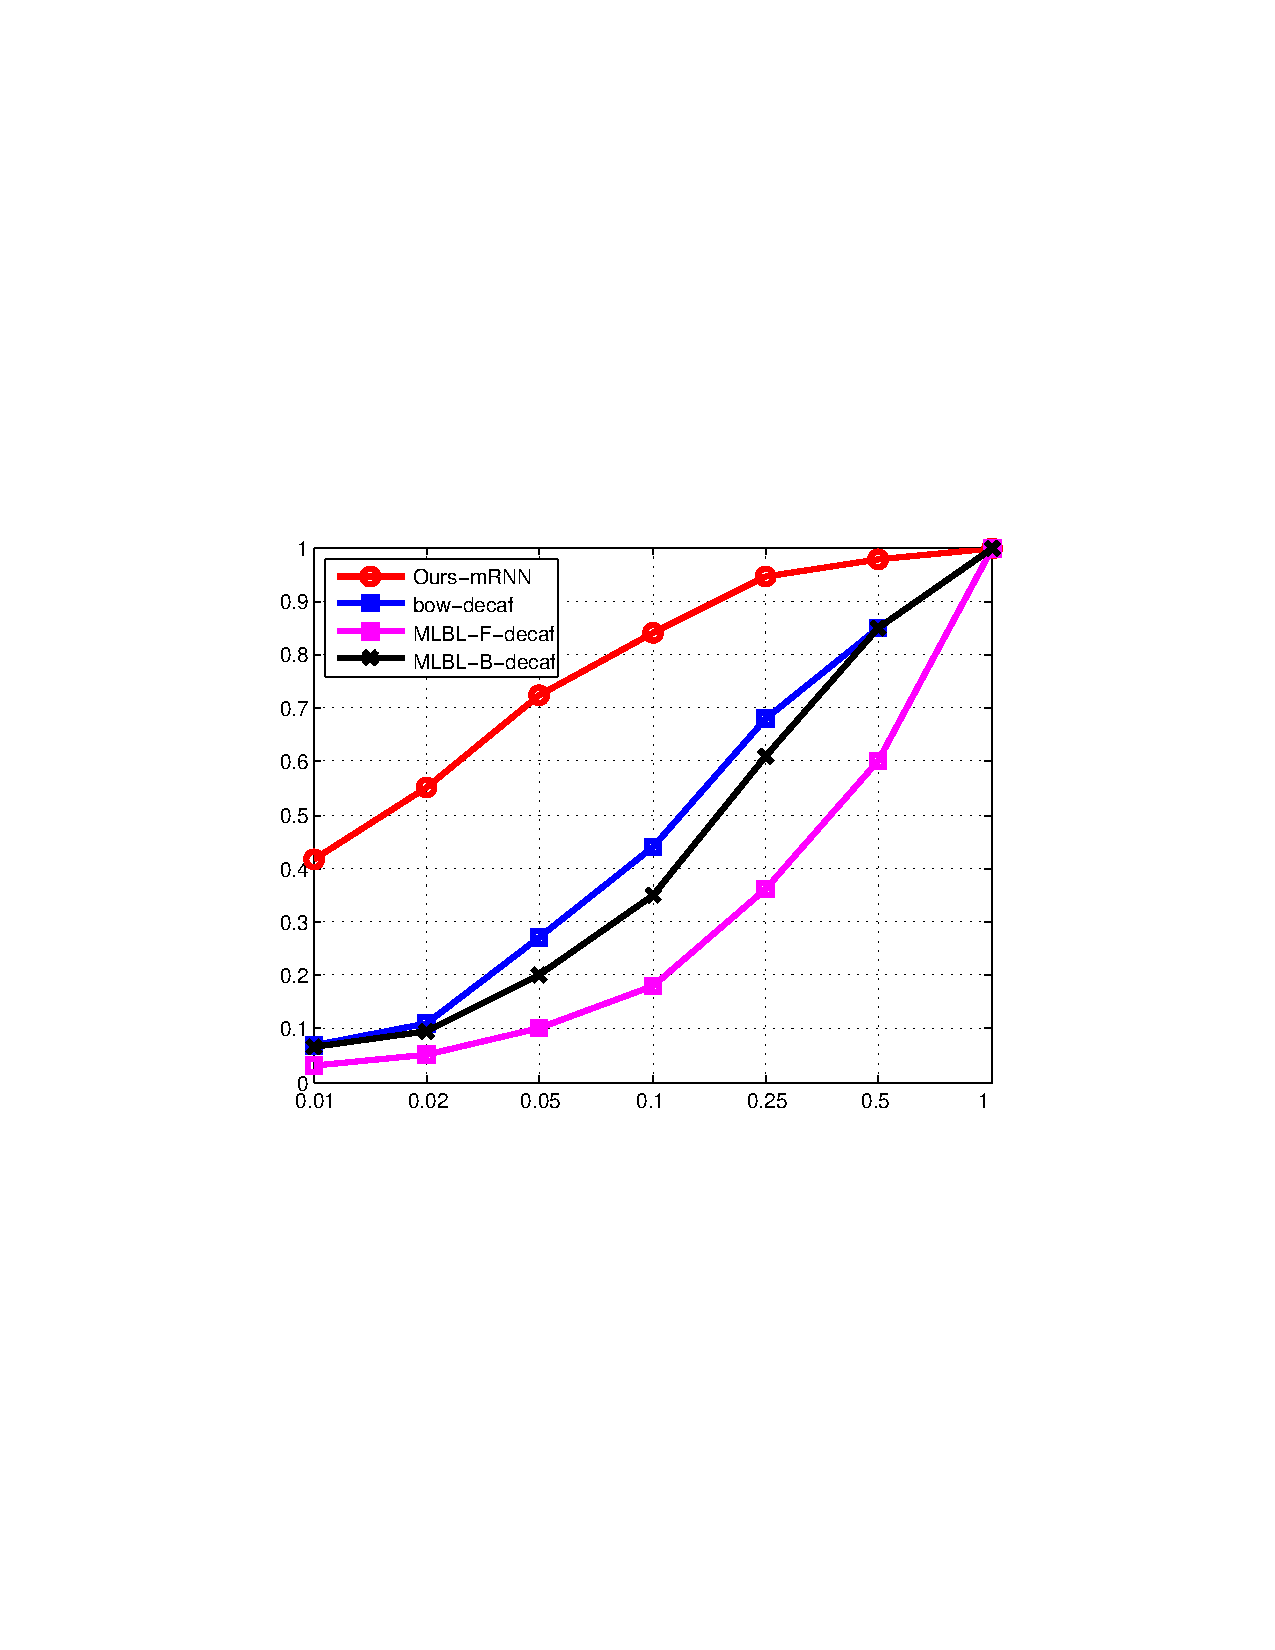
\includegraphics[width=\textwidth]{PaperFigures/I2T_iaprtc.pdf}
                \caption{Image to Text Curve}
        \end{subfigure}%
        ~ %add desired spacing between images, e. g. ~, \quad, \qquad, \hfill etc.
          %(or a blank line to force the subfigure onto a new line)
        \begin{subfigure}[b]{0.42\textwidth}
                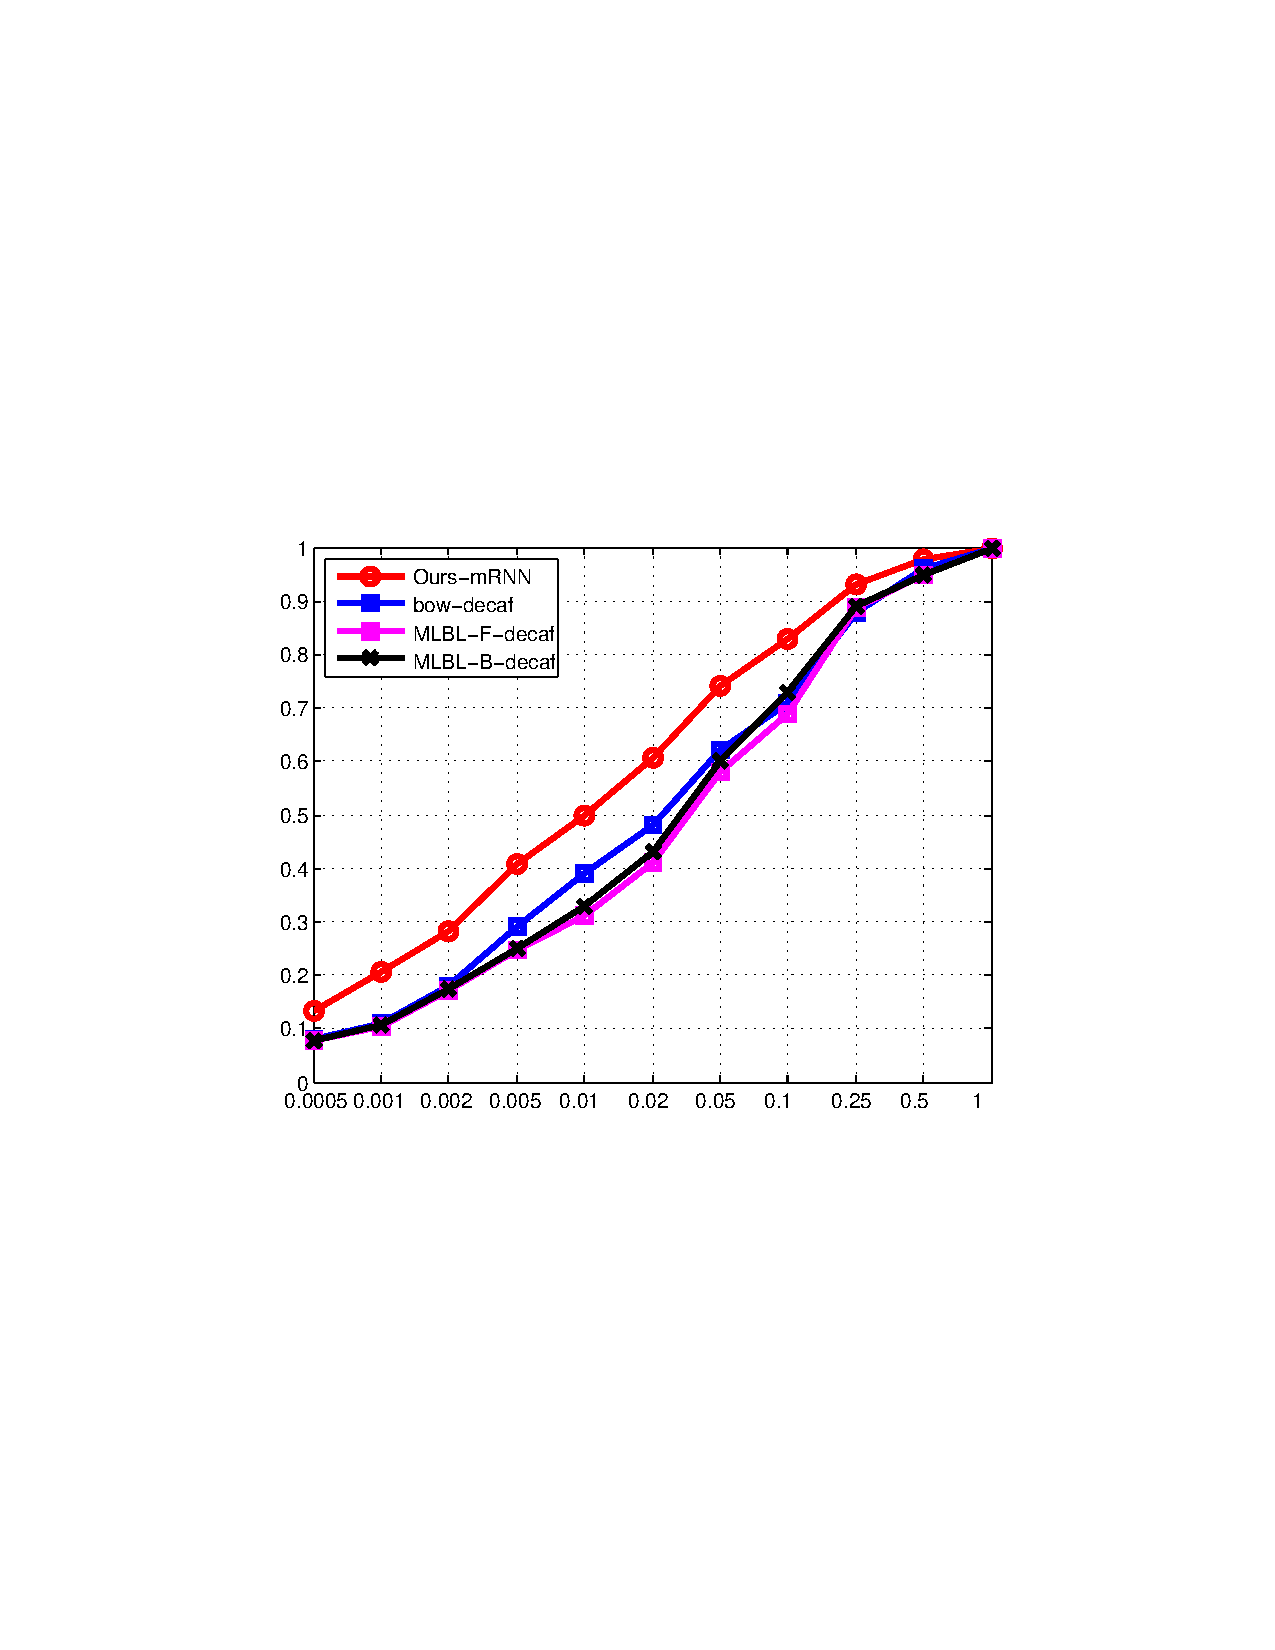
\includegraphics[width=\textwidth]{PaperFigures/T2I_iaprtc.pdf}
                \caption{Text to Image Curve}
        \end{subfigure}
        \caption{Retrieval recall curve for (a). Sentence retrieval task (Image to Text) (b). Image retrieval task (Text to Image) of iaprtc-12 dataset.}
        \label{fig:iaprtc_ret_curve}
\end{figure}

\begin{table}[htb]
	\centering
\begin{tabular}{l|cccc|cccc}
\hline
      & \multicolumn{4}{c|}{Sentence Retrival (Image to Text)} & \multicolumn{4}{c}{Image Retrival (Text to Image)} \\
\hline
      & R@1   & R@5   & R@10  & Med r & R@1   & R@5   & R@10  & Med r \\
\hline
Ours-m-RNN & 20.9  & 43.8  & 54.4  & 8     & 13.2  & 31.2  & 40.8  & 21 \\
\hline
\end{tabular}%
	\caption{Results of R@K and median rank (Med r) for iaprtc-12 dataset.}
	\label{tab:iaprtc_ret}
\end{table}

\subsection{Results on flickr8K}

This dataset was widely used for a benchmark dataset of Text to Image retrieval and Image to Text retrieval.
There are no publicly available methods that reports the statistics of generated sentences.

We first show the R@K evaluation metric in Table \ref{tab:flickr8K_ret}.
Our model outperforms the state-of-the-art methods (i.e Socher-decaf, DeViSE-decaf, DeepFE-decaf) by a large margin when using the same image features (i.e. decaf features).
In a recent work \cite{karpathy2014fragment}, they showed that using more sophisticated image features (e.g. decaf feature combined with detection results), will increase the performance.
We also list the result of the methods using such features in Talbe \ref{tab:flickr8K_ret}.
Socher-avg-rcnn and DeViSE-avg-rcnn used features of the average CNN activation of all objects above a detection confidence threshold \cite{karpathy2014fragment}.
DeepFE-rcnn used a image feature that further utilizes the RCNN detection algorithm.
Socher-avg-rcnn and DeepFE-rcnn all shows better results than their original version of Socher-decaf and DeepFE-decaf.
From the table, we can see that our method even performs better than these methods in most of the evaluation metrics.
We will develop our framework using the detection algorithm in the future work.

\begin{table}[htb]
	\centering
\begin{tabular}{l|cccc|cccc}
\hline
      & \multicolumn{4}{c|}{Sentence Retrival (Image to Text)} & \multicolumn{4}{c}{Image Retrival (Text to Image)} \\
\hline
      & R@1   & R@5   & R@10  & Med r & R@1   & R@5   & R@10  & Med r \\
\hline
Random & 0.1   & 0.5   & 1.0   & 631   & 0.1   & 0.5   & 1.0   & 500 \\
Socher-decaf \cite{socher2014grounded} & 4.5   & 18.0  & 28.6  & 32    & 6.1   & 18.5  & 29.0  & 29 \\
Socher-avg-rcnn \cite{socher2014grounded} & 6.0   & 22.7  & 34.0  & 23    & 6.6   & 21.6  & 31.7  & 25 \\
DeViSE-avg-rcnn \cite{frome2013devise} & 4.8   & 16.5  & 27.3  & 28    & 5.9   & 20.1  & 29.6  & 29 \\
DeepFE-decaf \cite{karpathy2014fragment} & 5.9   & 19.2  & 27.3  & 34    & 5.2   & 17.6  & 26.5  & 32 \\
DeepFE-rcnn \cite{karpathy2014fragment} & 12.6  & 32.9  & 44.0  & 14    & 9.7   & 29.6  & \textbf{42.5} & \textbf{15} \\
Ours-m-RNN-decaf & \textbf{14.5} & \textbf{37.2} & \textbf{48.5} & \textbf{11} & \textbf{11.5} & \textbf{31.0} & 42.4  & \textbf{15}\\
\hline
\end{tabular}%
	\caption{Results of R@K and median rank (Med r) for flickr8K dataset.}
	\label{tab:flickr8K_ret}
\end{table}

We also reports the results of generated sentences in Table \ref{tab:flickr8K_gen}.
There is no publicly available algorithm that reported results on this dataset.
We compared our m-RNN model with the Ours-RNN-Base model.
The m-RNN model performs much better than the baseline both in terms of the perplexity and BLEU scores.

\begin{table}[htb]
	\centering
\begin{tabular}{l|cccc}
\hline
      & PERP  & B-1   & B-2   & B-3 \\
\hline
Ours-RNN-Base & 30.39 & 0.4383 & 0.1849 & 0.1339 \\
Ours-m-RNN & \textbf{24.39} & \textbf{0.5778} & \textbf{0.2751} & \textbf{0.2307} \\
\hline
\end{tabular}%
	\caption{Results of generated sentences in the flickr8K dataset. }
	\label{tab:flickr8K_gen}
\end{table}

\subsection{Results on flickr30K}

This dataset is a new dataset and there are only a few methods report their retrieval results on it.
We first show the R@K evaluation metric in Table \ref{tab:flickr30K_ret}.
Our method outperforms the state-of-the-art methods in most of the evaluation metrics.

In addition, no publicly available methods reported the results of the sentence generation task as the best of our knowledge.
We report the results of generated sentences in Table \ref{tab:flickr30K_gen} with a comparison of our RNN baseline.

\begin{table}[htb]
	\centering
\begin{tabular}{l|cccc|cccc}
\hline
      & \multicolumn{4}{c|}{Sentence Retrival (Image to Text)} & \multicolumn{4}{c}{Image Retrival (Text to Image)} \\
\hline
      & R@1   & R@5   & R@10  & Med r & R@1   & R@5   & R@10  & Med r \\
Random & 0.1   & 0.6   & 1.1   & 631   & 0.1   & 0.5   & 1.0   & 500 \\
DeViSE-avg-rcnn \cite{frome2013devise} & 4.8   & 16.5  & 27.3  & 28    & 5.9   & 20.1  & 29.6  & 29 \\
DeepFE-rcnn \cite{karpathy2014fragment} & 16.4  & \textbf{40.2} & \textbf{54.7} & \textbf{8} & 10.3  & \textbf{31.4} & \textbf{44.5} & \textbf{13} \\
Ours-m-RNN-decaf & \textbf{18.4} & \textbf{40.2} & 50.9  & 10    & \textbf{12.6} & 31.2  & 41.5  & 16 \\
\hline
\end{tabular}%
	\caption{Results of R@K and median rank (Med r) for flickr30K dataset.}
	\label{tab:flickr30K_ret}
\end{table}

\begin{table}[h]
	\centering
\begin{tabular}{l|cccc}
\hline
      & PERP  & B-1   & B-2   & B-3 \\
\hline
Ours-RNN-Base & 43.96 & 0.4699 & 0.1964 & 0.1252 \\
Ours-m-RNN & \textbf{35.11} & \textbf{0.5479} & \textbf{0.2392} & \textbf{0.1952} \\
\hline
\end{tabular}%
	\caption{Results of generated sentences in the flickr8K dataset. }
	\label{tab:flickr30K_gen}
\end{table}